\documentclass{article}
\usepackage{graphicx}
\usepackage[margin=1.5cm]{geometry}
\usepackage{amsmath}

\begin{document}

\title{Warm Up: Unit 3, Forces}
\author{Prof. Jordan C. Hanson}

\maketitle

\section{Memory Bank}

\begin{enumerate}
\item $\vec{F}_{net} = \sum_i \vec{F}_i$ ... If $\vec{v} = 0$, Newton's First Law implies $\vec{F}_{net} = 0$.
\end{enumerate}

\begin{figure}[ht]
\centering
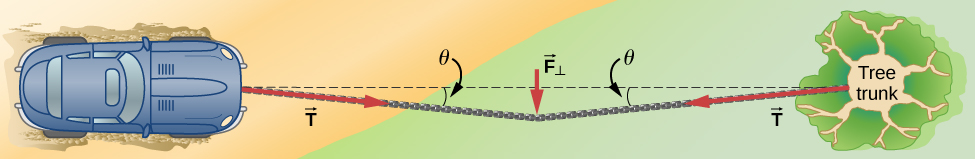
\includegraphics[width=0.75\textwidth]{rope.jpeg}
\caption{\label{fig:1} Person pushes in a direction orthogonal to a rope connecting a car and a tree.}
\end{figure}

\section{Chapter 5 - Forces}

\begin{enumerate}
\item If the force perpendicular to the rope, $\vec{F}_{\perp}$, and the left-pointing tension $\vec{T}$ and right-pointing tension $\vec{T}$ all cancel to yield $\vec{F}_{net} = 0$, show that
\begin{equation}
2T\sin\theta = F_{\perp}
\end{equation}
\textit{Hint: it helps if you think of the tension vectors as pointing the opposite direction as shown in Fig. 1.} \\ \vspace{3cm}
\item What is the tension in the rope if we find an angle $\theta = 10$ degrees, and $F_{\perp} = 500$ N?
\end{enumerate}

\end{document}
